\section{Anti-localization and SBT-legal data}
\label{sec:spt-legal}

\Cref{sec:no-go-icap} showed that localized admissible inputs make a uniform capacity certificate
as strong as a pointwise bound. This section states the restriction that removes those inputs,
proves that it follows from a channel structure, and turns it into a certificate that can be
computed on initial data.

The word ``SBT-legal'' is used in two senses. \emph{Analytically}, it names a restricted problem in
which the admissible interface inputs at each scale cannot concentrate. This is a hypothesis on
admissible signals, not a theorem about Navier--Stokes. \emph{Operationally}, it names a certificate
that tests this restriction at a chosen resolution and time window. We use the certificate on
initial data and as a diagnostic along short runs. We do not claim that passing it at $t=0$ implies
passing it later; that persistence question is open (\cref{sec:discussion}).

\subsection{Anti-localization}

Fix a shell $j$ and let $B_j(x_0)$ be a ball of radius comparable to $2^{-j}$. The \emph{worst local
energy fraction} of $u$ in shell $j$ is
\begin{equation}\label{eq:local-energy-fraction}
L_j(u):=\sup_{x_0\in\T^3}\frac{\int_{B_j(x_0)}|u_j(x)|^2\,dx}{\|u_j\|_{L^2}^2}\in[0,1],
\end{equation}
with the convention $L_j(u)=0$ when $u_j=0$.

\begin{definition}[Anti-localization at scale $j$]\label{def:anti-localization}
A shell field $v\in\mathrm{Ran}(\Delta_j)$ is \emph{$\eta_j$-anti-localized} if
\begin{equation}\label{eq:antiloc}
\sup_{x_0\in\T^3}\int_{B_j(x_0)}|v(x)|^2\,dx\ \le\ \eta_j\,\|v\|_{L^2}^2 .
\end{equation}
A family of shell classes is \emph{asymptotically anti-localized} if this holds with $\eta_j\to0$.
\end{definition}

The inequality needs no division, so it is meaningful for $v=0$. If $\eta_j\to0$, then at large $j$
no admissible input can keep a fixed fraction $c_0>0$ of its energy in one ball $B_j(x_0)$: once
$\eta_j<c_0$, the localized tests of \cref{sec:no-go-icap} are excluded. This blocks that
particular argument. It provides no capacity bound, no work quantum and no divergence by itself.

\subsection{Few spread-out channels force anti-localization}

One way to obtain anti-localization is \emph{channelization}: admissible shell inputs are
combinations of a few channel shapes, each spread out in space. An interface that exposes only a
few delocalized degrees of freedom cannot target a single cell. The following lemma is stated in a
finite model, as it is mechanized.

\begin{lemma}[Delocalized channels give anti-localization]\label{lem:channel-antiloc}
Let $\rho$ be a finite set of $m$ channels, $\iota$ a finite set of grid cells, and $B\subset\iota$
one cell group. Let the channel shapes $\psi_r:\iota\to\R$ satisfy
\[
\sum_{i\in B}\psi_r(i)^2\ \le\ \kappa\,\mu(B)\qquad\text{for every }r\in\rho,
\]
with $\kappa\ge0$ and $\mu(B)\ge0$. Then every synthesized field $u=\sum_r a_r\psi_r$ satisfies
\begin{equation}\label{eq:finite-channel-antiloc}
\sum_{i\in B}u(i)^2\ \le\ m\,\kappa\,\mu(B)\sum_{r\in\rho}a_r^2 .
\end{equation}
If the channels are orthonormal, $\sum_i\psi_r(i)\psi_s(i)=\delta_{rs}$, then
$\sum_{i\in\iota}u(i)^2=\sum_ra_r^2$, and therefore
$\sum_{i\in B}u(i)^2\le m\,\kappa\,\mu(B)\sum_{i\in\iota}u(i)^2$.
\end{lemma}

\begin{proof}
Pointwise, $u(i)^2\le m\sum_r a_r^2\psi_r(i)^2$ by Cauchy--Schwarz. Summing over $B$ and using the
channel bound gives \eqref{eq:finite-channel-antiloc}. For orthonormal channels, expanding the square
and using the Gram identity gives Parseval.
\end{proof}

The bound holds for the cell group $B$ named in the hypothesis. A bound uniform over all cells, as
in \eqref{eq:antiloc}, needs the channel hypothesis for every cell. Lean proves the coefficient
form (\nolinkurl{mass_cell_le_card_mul_deloc_mul_coeffEnergy}), the Parseval identity from the Gram
matrix (\nolinkurl{synthesis_energy_eq_coeffEnergy_of_orthonormal}) and the field-energy form
(\nolinkurl{mass_cell_le_card_mul_deloc_mul_fieldEnergy_of_orthonormal}), all in
\nolinkurl{formal/Fluids/AntiLocalization.lean}. The continuum version, with $L^2$ integrals over
balls, follows from the same Cauchy--Schwarz argument and gives $\eta_j\le m_j\kappa\,\mu(B_j)$.

\paragraph{Scaling.}
A ball of radius $c\,2^{-j}$ occupies a volume fraction $\mu(B_j)\sim2^{-3j}$ of $\T^3$. With $\kappa$
fixed, the returned constant $\eta_j\le m_j\kappa\,2^{-3j}$ tends to zero exactly when
$m_j2^{-3j}\to0$, for example when $m_j\lesssim j+1$. A finite channel count at each depth is not
enough without this growth condition.

\subsection{Measured channels and their residual}

In practice the channels are estimated from data, for example as the leading singular vectors of a
matrix of shell snapshots. A measured span need not contain the data exactly, and the part left out
can itself be localized. The following elementary bound charges it.

\begin{lemma}[Residual-charged anti-localization]\label{lem:residual}
Let $\eta\ge0$ and let $u=v+r\ne0$, where $v$ lies in a channel span whose fields satisfy
\eqref{eq:antiloc} with constant $\eta$, and $r\perp v$ in $L^2$. Write $\delta=\|r\|_{L^2}^2/\|u\|_{L^2}^2$.
Then for every ball $B=B_j(x_0)$ of the family in \eqref{eq:antiloc}
\[
\frac{\int_B|u|^2}{\|u\|_{L^2}^2}\ \le\ \min\Bigl(1,\ \bigl(\sqrt{\min(\eta,1)\,(1-\delta)}+\sqrt\delta\bigr)^2\Bigr).
\]
\end{lemma}

\begin{proof}
By the triangle inequality in $L^2(B)$,
$\|u\|_{L^2(B)}\le\|v\|_{L^2(B)}+\|r\|_{L^2(B)}\le\sqrt{\min(\eta,1)}\,\|v\|_{L^2}+\|r\|_{L^2}$, and
orthogonality gives $\|v\|_{L^2}^2=(1-\delta)\|u\|_{L^2}^2$.
\end{proof}

The returned bound tends to zero when both $\eta_j\to0$ for the span and $\delta_j\to0$ for the
residual. These are sufficient conditions for this bound, not necessary ones for the actual fields:
a residual can carry a fixed fraction of the energy and still be spread out. A rank that retains a
fixed $95\%$ of pooled snapshot energy controls neither quantity. It bounds the residual of the pooled data, not of each snapshot, and a small
residual can be concentrated.

\subsection{An operational certificate}

We now define the computable notion used in the experiments. It is an admissibility filter for a
restricted research question, not a criterion for the Clay problem: \emph{do SBT-legal data evolve
without Zeno cascades?}

\begin{definition}[SBT-legality certificate]\label{def:spt-legal-cert}
On an $N^3$ grid, for each shell $j$ let $L_j$ be the largest fraction of the shell-$j$ energy found
in a periodic grid cube of side $w_j=\mathrm{round}(N/2^j)$ cells (zero for an empty shell), and let
$f_j=(w_j/N)^3$ be the volume fraction of that cube. The \emph{concentration factor} is
\[
\kappa_j:=L_j/f_j ,
\]
so a perfectly uniform shell has $\kappa_j=1$ and a shell concentrated in one cube has
$\kappa_j=1/f_j$. Over a set of snapshots the certificate records $\max_t\kappa_j$, a \emph{burst
ratio} (the largest snapshot value of $L_j$ divided by its mean over snapshots, zero for a shell
that is empty in every snapshot) and, optionally, the
number $m_{95}$ of singular vectors needed to retain $95\%$ of the pooled, uncentered snapshot
energy. A field is \emph{SBT-legal at thresholds} $(\kappa_\star,\mathrm{burst}_\star,m_\star)$ if
every recorded statistic is valid and at most its threshold.
\end{definition}

The certificate uses grid cubes, whereas \eqref{eq:antiloc} uses balls; comparing their constants
requires a geometric adapter. The certificate tool (\nolinkurl{ns_spt_legal_certify.py}; file names
use the abbreviation ``spt'') writes a machine-readable JSON record with its configuration. It
rejects invalid input instead of passing it: nonfinite or non-real spectra, inconsistent shell
counts, factors that are not the stated ratio of raw fraction to baseline, and missing or
non-integer ranks when ranks are required.

\subsection{The certificate is not vacuous}

A legal baseline and an illegal construction make the point. The baseline is a smooth random
band-limited field of the kind used throughout the demos. The illegal field is a divergence-free
blob placed in a single dyadic shell ($j=3$) and concentrated near one point
(\nolinkurl{illegal_initial_conditions.py}), rescaled to the energy of the baseline. Band-limiting alone does not prevent concentration: the
illegal field is band-limited by construction.

\begin{figure}[t]
  \centering
  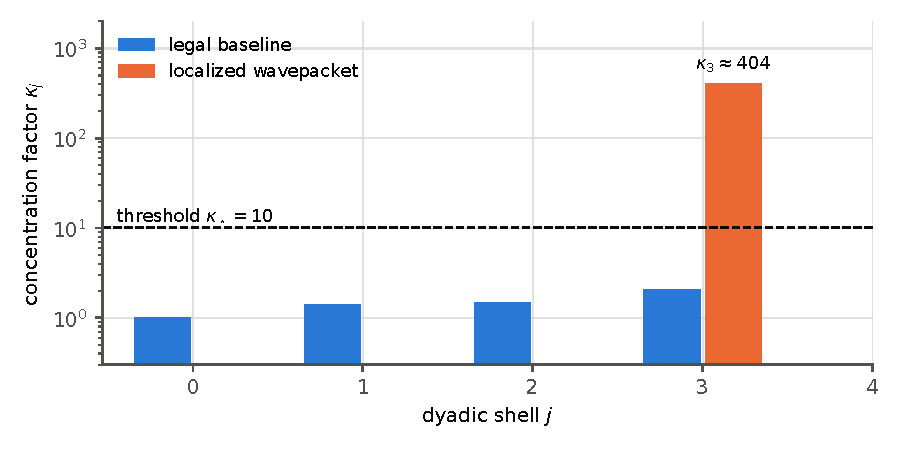
\includegraphics[width=0.82\linewidth]{figures/spt_illegal_vs_legal.pdf}
  \caption{\textbf{Legal and illegal initial data under the same certificate} ($N=32$, $t=0$).
  The legal baseline has $\kappa_j$ between 1.0 and 2.1 in every occupied shell. The localized
  wavepacket in shell $j=3$ reaches $\kappa_3\approx404$, forty times the threshold
  $\kappa_\star=10$. The shell $j=4$ is empty in both fields, because the baseline is band-limited to $|k|\le10$ and
the illegal field occupies only $j=3$; empty shells are reported as zero.
  Note the logarithmic scale.}
  \label{fig:spt-illegal-vs-legal}
\end{figure}

\begin{remark}[What this does not claim]
We do not prove that Navier--Stokes preserves SBT-legality, nor that every smooth initial datum is
legal. Anti-localization is one proposed way to avoid the obstruction of \cref{thm:icap-no-go};
the theorem does not show that it is the only one. Here we state that hypothesis precisely, mechanize its finite
inequality logic, and provide a reproducible certificate that tests it on concrete data.
\end{remark}
